\documentclass[12pt, a4paper]{AnantDocumentation}

\title{EEE F435: Digital Image Processing \\ Assignment 2}
\author{Pranav Chandra N. V. \\ 2023AAPS0013P}
\date{29th September, 2025}
\backgroundsetup{
	contents = ""
}

\usepackage[T1]{fontenc}
\usepackage{listings}
\lstset{
	backgroundcolor=\color{white},
	basicstyle=\ttfamily\small,
	breaklines=true,
	frame=single,
	numbers=left,
	numberstyle=\tiny,
	keywordstyle=\color{blue},
	commentstyle=\color{gray},
	stringstyle=\color{red},
	showstringspaces=false
}

\begin{document}
\maketitle
\tableofcontents
\newpage
\listoffigures

\newpage

\section{Introduction}
The goal of this assignment was to work with the functions that are used for operations in the frequency domain. All code was done in MATLAB, some of this code is provided in the appendix, with snippets provided within the main body to maintain brevity and flow. Two images were used, one from the first assignment, and the second taken recently for this assignment. In some cases, both images have been used, while in others, only one has been used (for simplicity's sake).	

All images were converted to grayscale, and both images were resized to the same size to allow all operations (especially in Task \ref{subsec:swapping magnitude and phase}). The entire code base can be found appended to the end of this report, following the guidelines provided in the assignment brief.

\section{Task 1}
This part was basic frequency domain operations on images, using the fast fourier transform operation within MATLAB.

\subsection{Image Frequency Domain Display}
\label{subsec:image frequency domain display}
Both sample images have been imported and shown here. In order to display the frequency domain aspects, the \lstinline[language=matlab]|fft| class of commands was used. In all cases, \lstinline[language=MATLAB]|fft2| was used, as we're working with 2D images here. Figure \ref{fig:displaying mag and phase of image}

\begin{lstlisting}[language=matlab]
	fft_1 = fft2(img_1);
	fftshift_1 = fftshift(fft_1);
	mag_1 = log(1 + abs(fftshift_1));
	phase_1 = angle(fftshift_1);
\end{lstlisting}
\begin{figure}[h!]
	\centering
	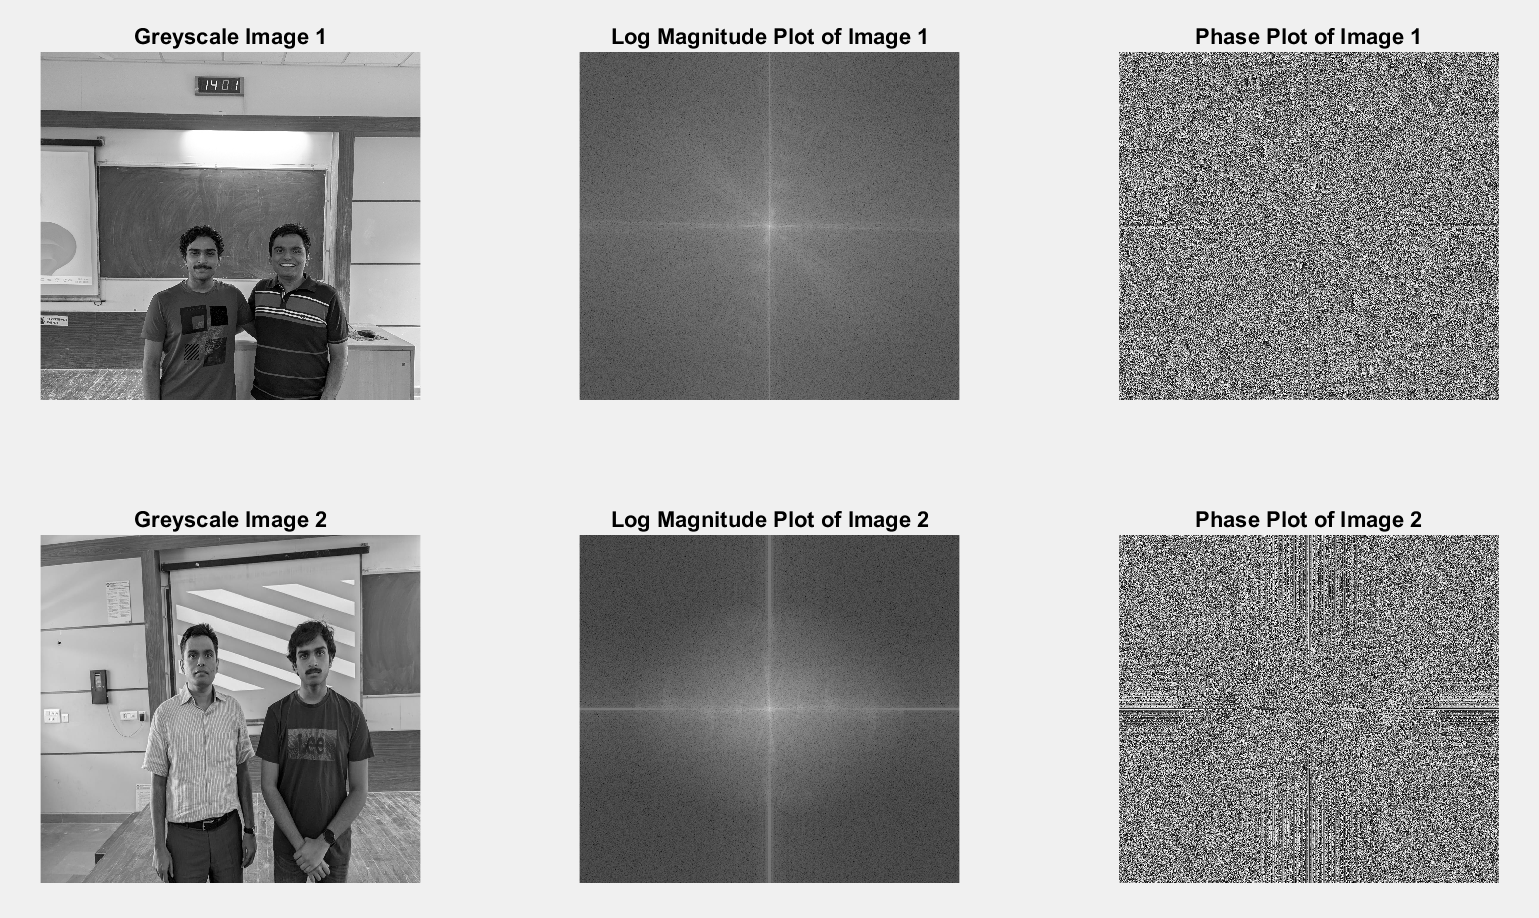
\includegraphics[width=0.9\textwidth]{images/task1-part1.png}
	\caption{Images in Time and Frequency Domain}
	\label{fig:displaying mag and phase of image}
\end{figure}

\subsection{Swapping Magnitude and Phase}
\label{subsec:swapping magnitude and phase}
When swapping the magnitude and phase of the two images, the most important consideration was to make sure that both the images were the same size. To do this, the \lstinline[language=MATLAB]|imresize| command was used. 

To swap the magnitudes and phase, the $a + jb = |M|e^{angle}$ property was used with the following code.

\begin{lstlisting}[language=matlab]
	mixed_1 = mag_1 .* exp(1i * phase_2);   
	mixed_1 = ifft2(ifftshift(mixed_1));    
	mixed_2 = mag_2 .* exp(1i * phase_1);
	mixed_2 = ifft2(ifftshift(mixed_2));
\end{lstlisting}

The resulting images are shown in Figure \ref{fig:swapping magnitude and phase}. 

\begin{figure}[h!]
	\centering
	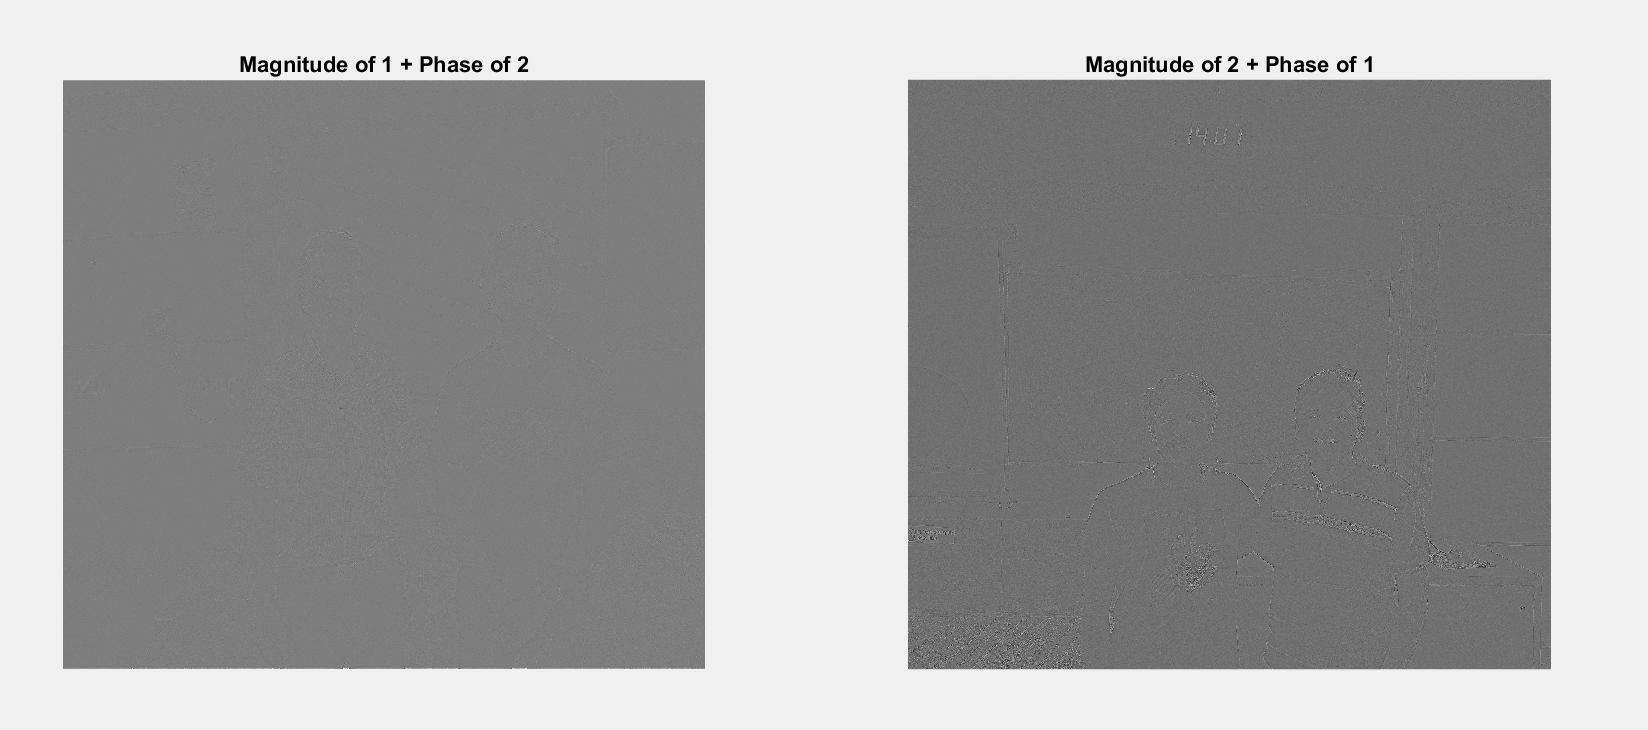
\includegraphics[width=\textwidth]{images/task1-part3.png}
	\caption{Images 1 and 2 with swapped magnitudes}
	\label{fig:swapping magnitude and phase}
\end{figure}
 It can be observed that the image with the phase of image 1 and magnitude of image 2 looks more like image 1, while the other image looks more like image 2. This shows that the phase component of an image is more important than the magnitude component. 


\subsection{Shifting of Image}
\label{subsec:shifting of image}
Here, we had to shift the imgae. Shifting the image can be done in two ways. Using the \lstinline[language=MATLAB]|circshift| command, or using the \lstinline[language=MATLAB]|imtranslate| command. There is a stark difference in how these commands work, so the explanation has been divided into the subsequent two subsections.
 
\subsubsection{Circular Shifting}
\label{subsubsec:circular shifting of image}
The first tried test was circular shifting. The image was shifted to the right and down by the appropriate amounts, and the parts that were shifted out simply got shifted to the top and left of the image. 
\begin{lstlisting}[language=MATLAB]
shift_x = A * 10 + 5;
shift_y = B * 10 + 5;
img_1_shifted = circshift(img_1, [shift_y, shift_x]);
img_2_shifted = circshift(img_2, [shift_y, shift_x]);
\end{lstlisting}
The resulting images are shown in Figure \ref{fig:circular shifting of image}.
\begin{figure}[h!]
	\centering
	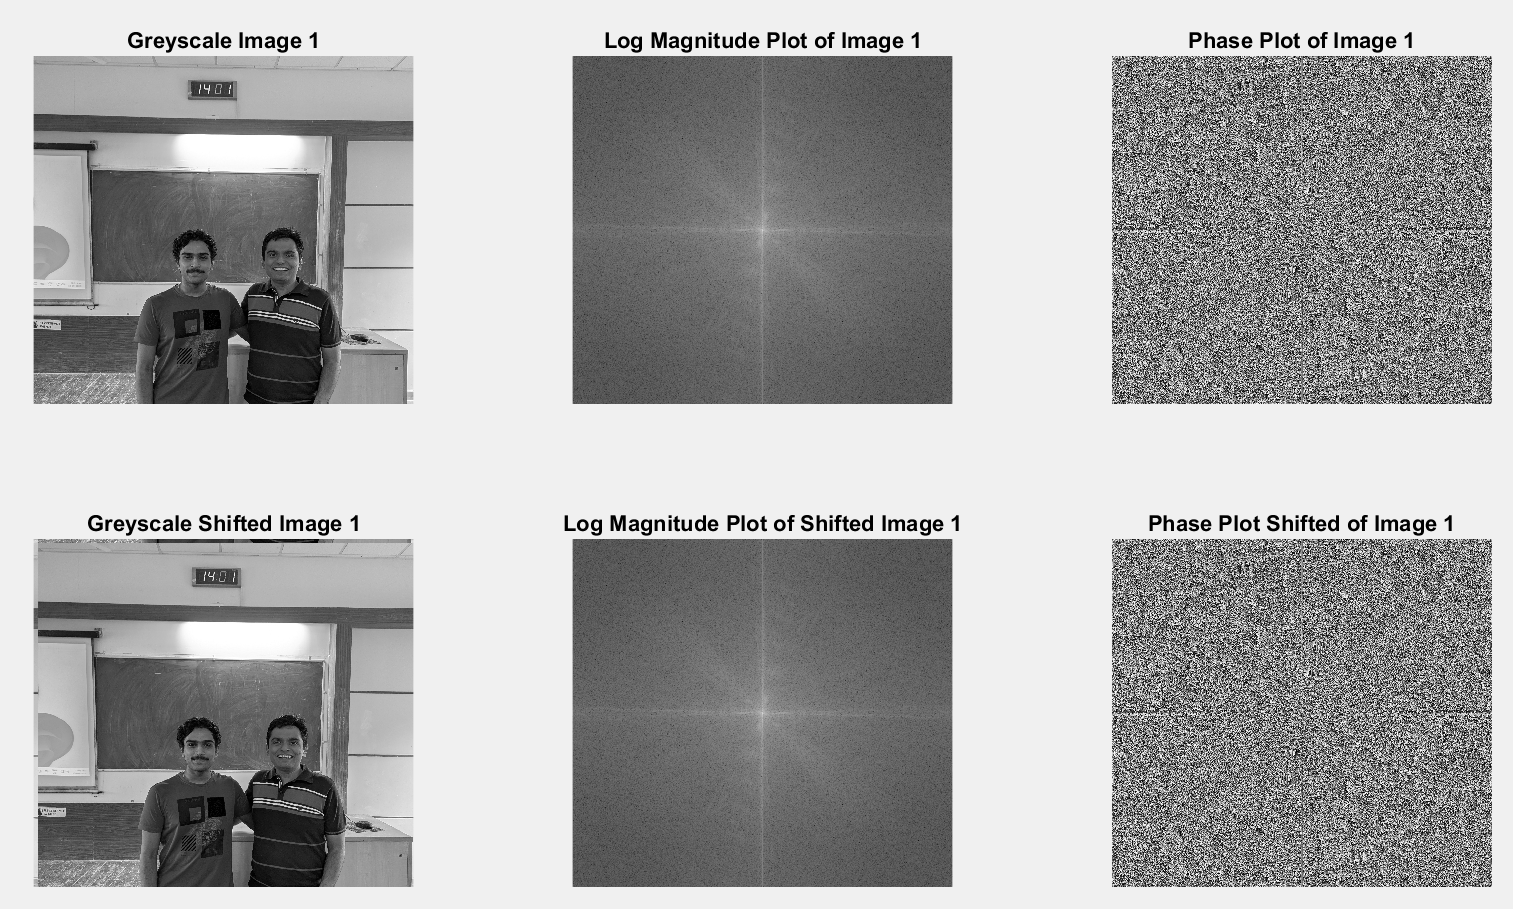
\includegraphics[width=\textwidth]{images/task1-part4.png}
	\caption{Circularly Shifted Images with Magnitude and Phase}
	\label{fig:circular shifting of image}
\end{figure}
 Unfortunately, the shifting is very small so not very visible unless you zoom in to the corners. However, in the frequency domain, an important fact emerges. Circular shifting causes no change in the frequency domain representation of the image. This is because circular shifting is equivalent to a periodic extension of the image, which does not affect its frequency components.

%TODO
\subsubsection{Translation of Image}
\label{subsubsec:translation of image}
The second method used was translation. This is done using the \lstinline[language=MATLAB]|imtranslate| command. This command shifts the image, and fills in the parts that are shifted out with a default value (0, black).

\subsection{Scaling of Image}
\label{subsec:scaling of image}
This task required us to scale the image. For brevity, only one image was scaled in accordance with the guidelines. The \lstinline[language=MATLAB]|imresize| command was used to perform this modification.

\begin{figure}[h!]
	\centering
	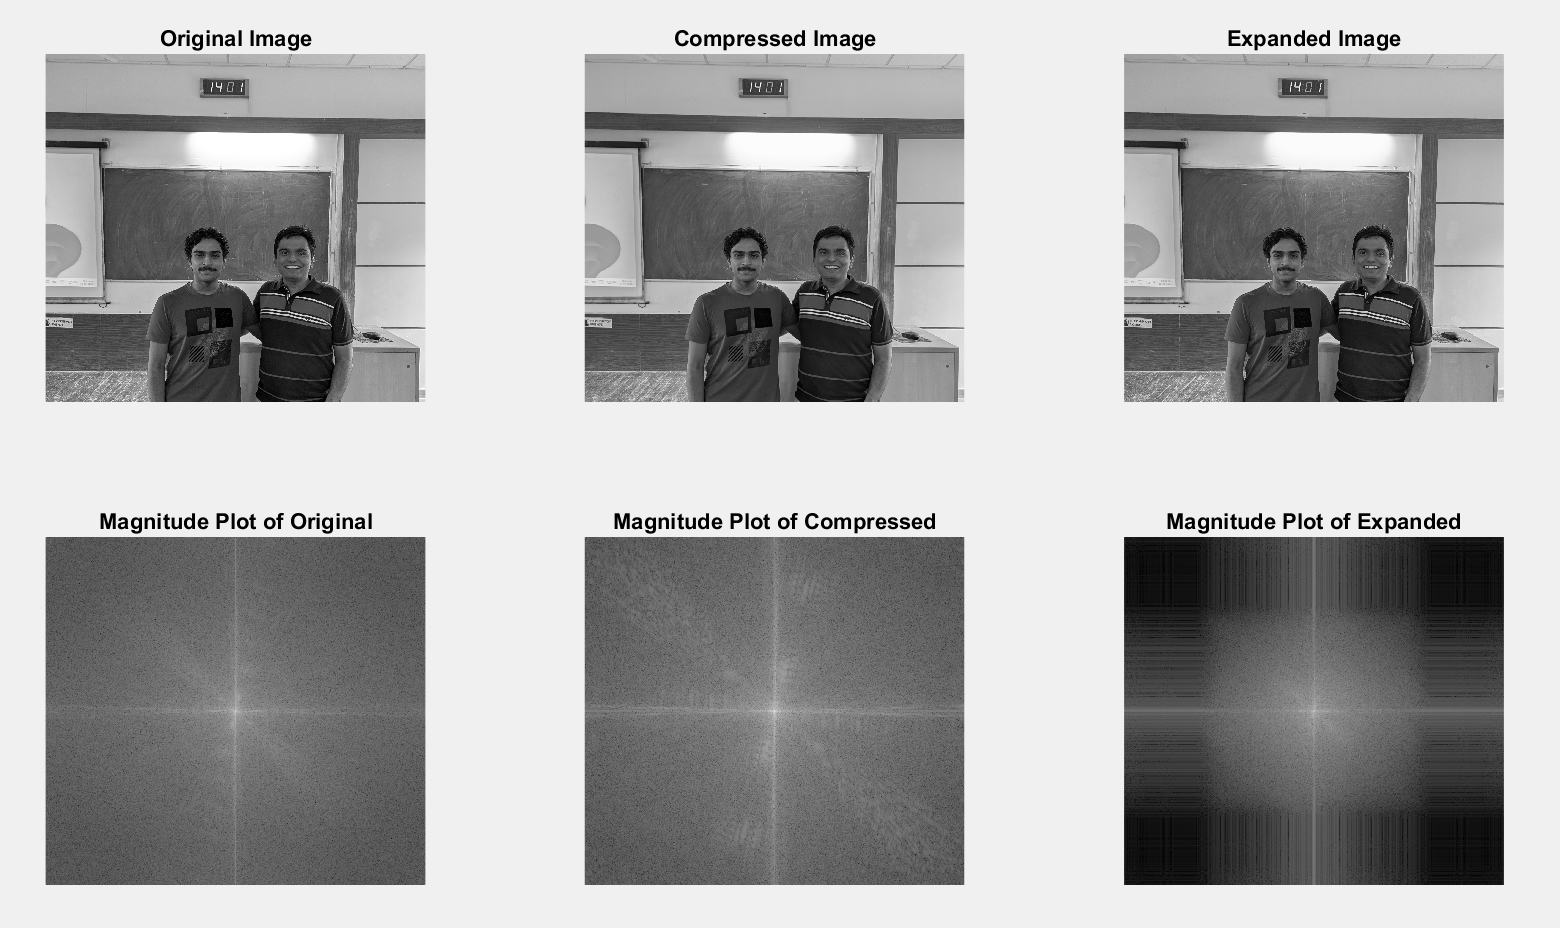
\includegraphics[width=\textwidth]{images/task1-part5.png}
	\caption{Scaled Image with Magnitude and Phase}
	\label{fig:scaled image}
\end{figure}

Figure \ref{fig:scaled image} shows the scaled image, along with its magnitude plot. 
It can be seen that the scaling causes a change in the magnitude plot. However, the scale down effect cannot be seen at this resolution, but the effect of scale up on magnitude is very clear. 


\subsection{Rotation of Image}
\label{subsec:rotation of image}
For the rotation of the image, the \lstinline[language=MATLAB]|imrotate| command was used. This command rotates the image by a specified angle, and fills in the parts that are rotated out with a default value (0, black). 
A simple for loop was used to generate the images at various angles, shown below.
\begin{lstlisting}[language=python]
angles = [0, 30, 45, 60, 90];
figure();
for k = 1:length(angles)
    theta = angles(k);
    img_rot = imrotate(img2, theta, 'bilinear', 'crop'); 
    
    F = fftshift(fft2(img_rot));
    mag = log(1 + abs(F));
    
    subplot(2, 5, k);
    imshow((img_rot));
    title(['Image after ', num2str(theta), ' rotation']);
    subplot(2, 5, k+5);
    imshow(mag, []);
    title(['Magnitude at ', num2str(theta), ' rotation']);
end
\end{lstlisting}

\begin{figure}[h!]
	\centering
	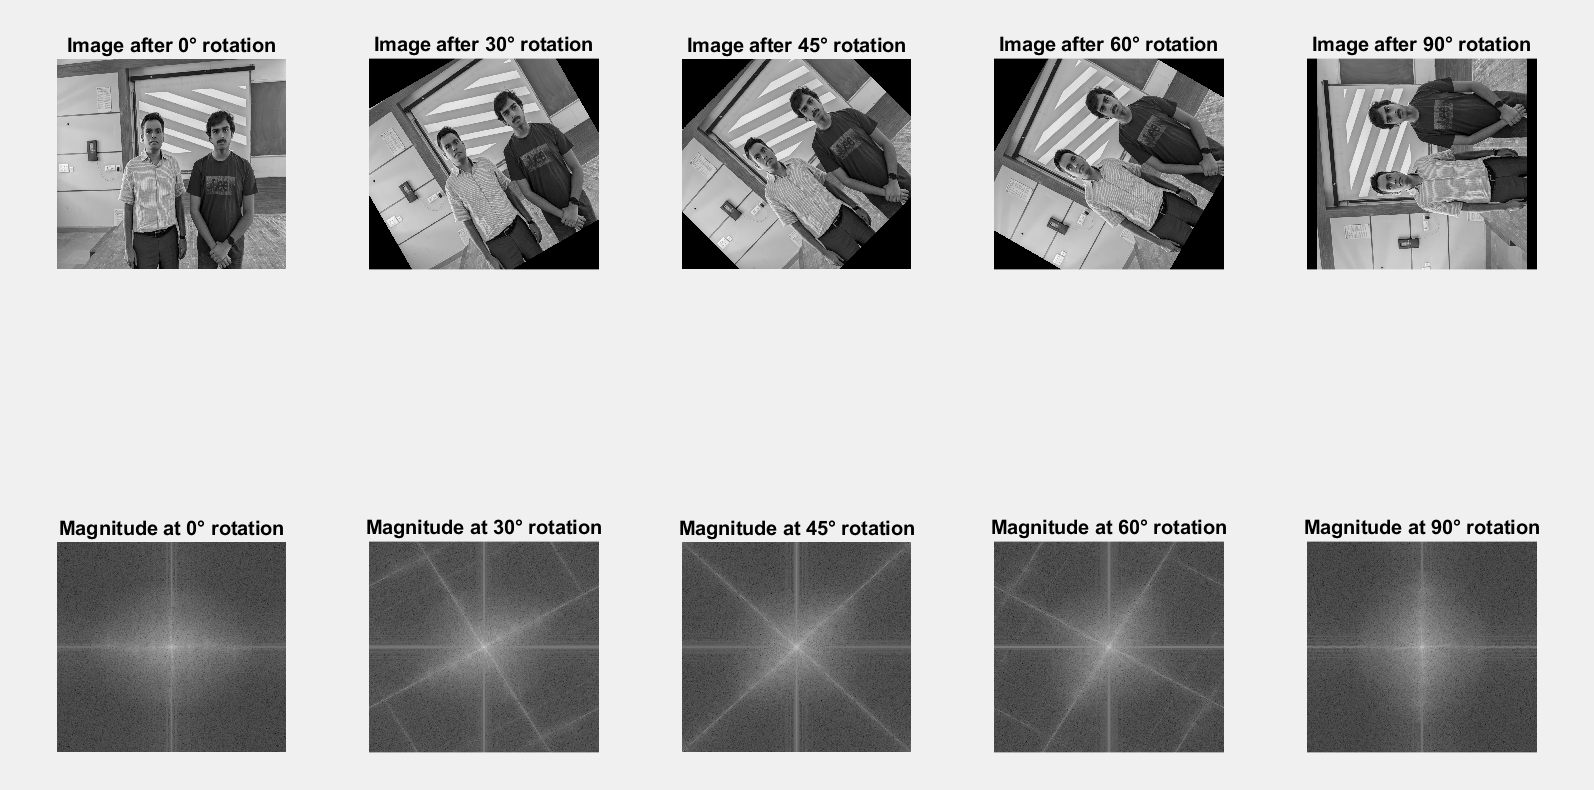
\includegraphics[width=\textwidth]{images/task1-part6.png}
	\caption{Image rotated by various angles}
	\label{fig:rotated images}
\end{figure}

It can be seen that the rotation in the time domain also causes a rotation in the freuqency domain plot.

\newpage
\section{Task 2 - Filters}
\label{sec:task 2 - filters}
In this section, we move towards applying a variety of filters on the image.
Both LPF and HPF filters are used. For all LPF filters, image 1 was used as a demo, and for all HPF filters, image 2 was used.

\subsection{Ideal LPF}
The ideal low pass filter is defined as:
\begin{equation}
	D(u, v) = \begin{cases}
		1 \hspace*{5mm} D(u, v) < R_0 \\
		0 \hspace{5mm} D(u, v) > R_0
	\end{cases}
\end{equation}
This filter only acts on the frequency domain. 
To identify the effects of a radial ideal LPF, radii 20, 50 and 100 pixels were chosen, and then applied. Once applied on the frequency domain, the image was converted back to time domain using the \lstinline[language=python]|ifft2| command.

To efficiently generate them, a quick for loop was used. Very similar code was used for the rectangular LPF.
\begin{lstlisting}[language=python]
radii = [20, 50, 100];  
for k = 1:length(radii)
    H = dist1 <= radii(k); % circular mask

    F1_filt = fft_shifted_1 .* H;
    img1_filt = real(ifft2(ifftshift(F1_filt)));
    imgs1{end+1} = img1_filt;
    F1s{end+1}   = F1_filt;
end
\end{lstlisting}

\newpage
The magnitude and phase plots of these circular LPF images were taken, and shown in Figure \ref{fig:circular lpf}.
\begin{figure}[h!]
	\centering
	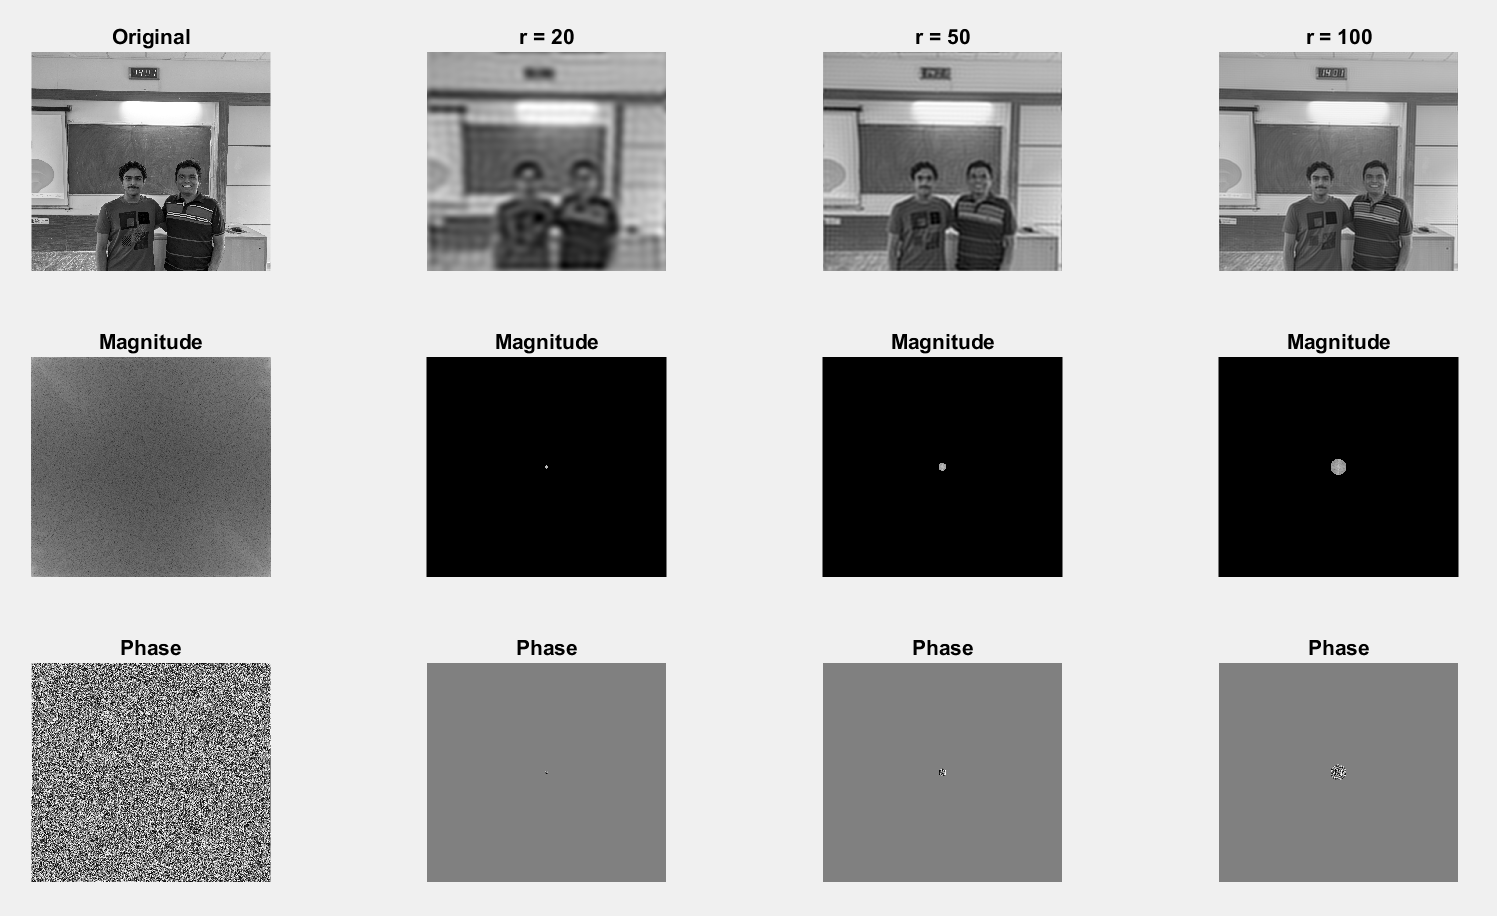
\includegraphics[width=0.9\textwidth]{images/task2-part1-circular.png}
	\caption{Circular LPF of Various Sizes}
	\label{fig:circular lpf}
\end{figure}

Now, for the rectangular LPF, the same process was used. The resultant images can be found in Figure \ref{fig:rectangular lpf}.
\begin{figure}[h!]
	\centering
	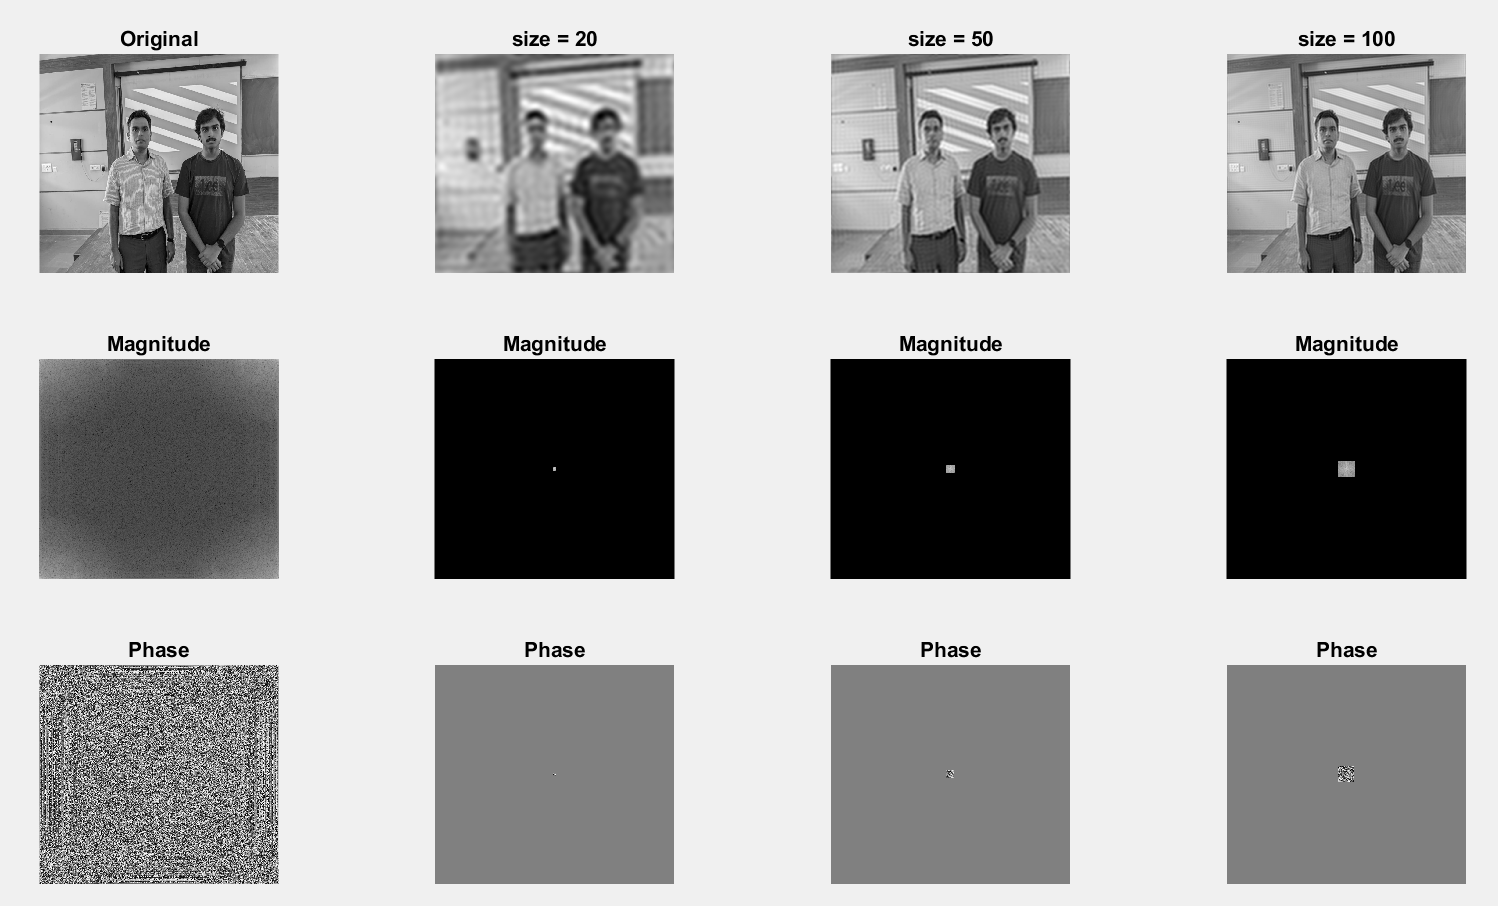
\includegraphics[width=0.9\textwidth]{images/task2-part1-rectangular.png}
	\caption{Rectangular LPF of Various Sizes}
	\label{fig:rectangular lpf}
\end{figure}

\subsection{Butterworth LPF}
\label{subsec:butterworth lpf}
The butterworth LPF is mathematically defined as:
\begin{equation}
	H(u, v) = \frac{1}{1 + \left(\frac{D(u, v)}{D_0}\right)^{2n}}
\end{equation}
Where $D_0$ is the cutoff frequency, and $n$ is the order of the filter. For this assignment, $n = 1, 2, 4$ was used. The same radii as before were used, and the results are shown in Figure \ref{fig:butterworth lpf}.
\begin{figure}[h!]
	\centering
	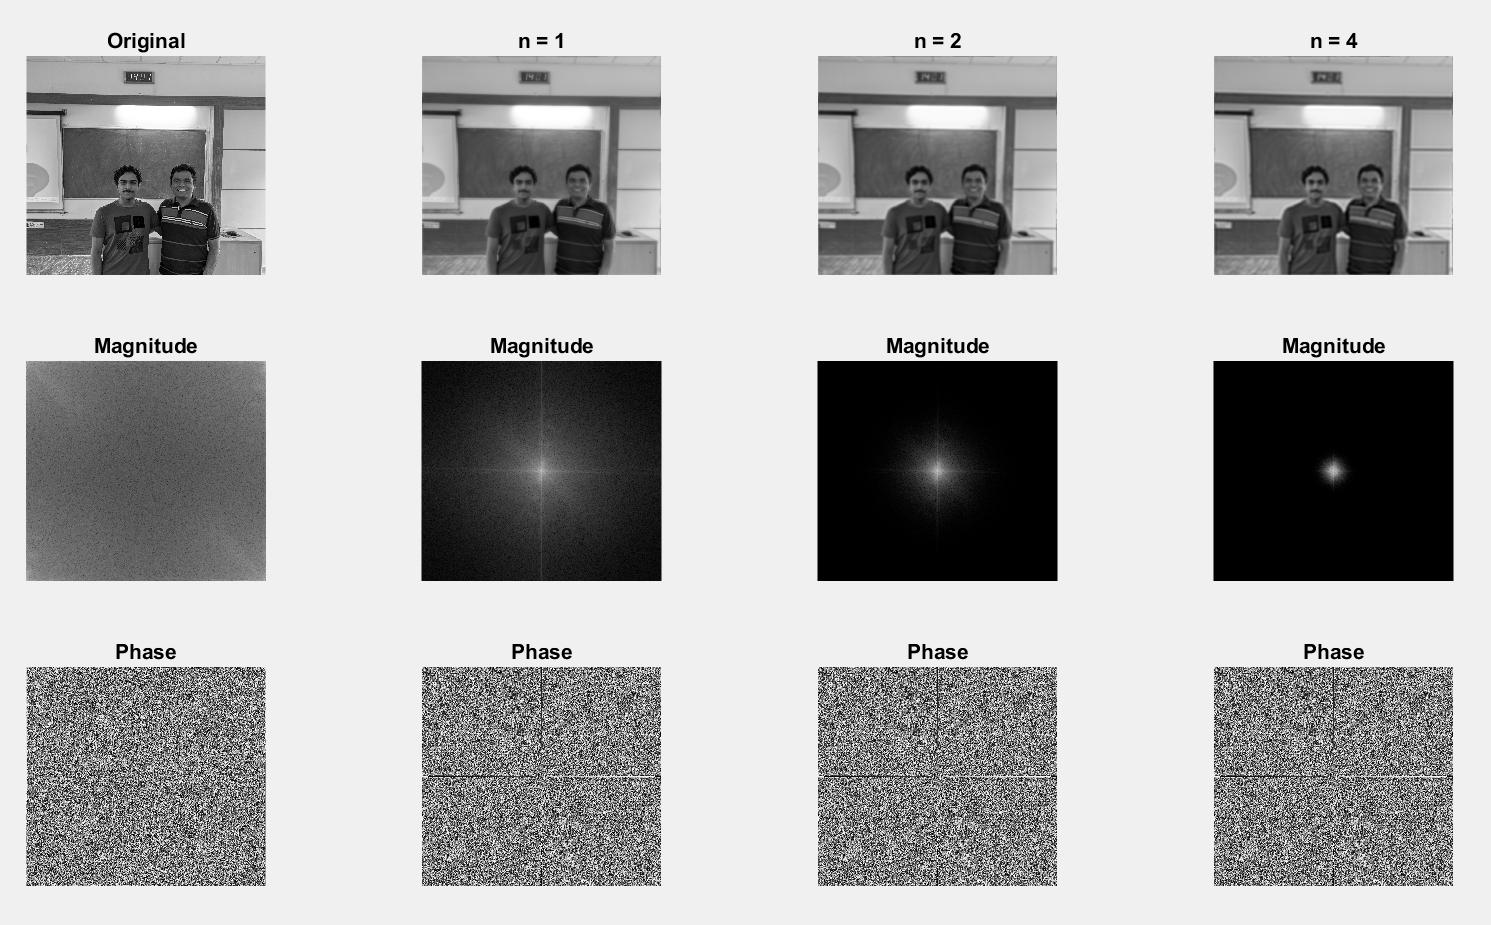
\includegraphics[width=\textwidth]{images/task2-part2.png}
	\caption{Butterworth Filtered Images of Various Orders and Sizes}
	\label{fig:butterworth lpf}
\end{figure}

The implementation in matlab was very simple, and very similar to the previous code. \lstinline[language=python]|H| was just changed as shown below.

\begin{lstlisting}[language=python]
H = 1 ./ (1 + (D./D0).^(2*n));
F_filt = fft_shifted_1 .* H;
img_filt = real(ifft2(ifftshift(F_filt)));
\end{lstlisting}

Higher frequency components from the image were removed as the order of the butterworth filter was increased, this can be seen in both the magnitude graph, and the images, where noisy bands were removed.

\newpage
\subsection{Gaussian LPF}
\label{subsec:gaussian lpf}
The Gaussian LPF is mathematically defined as:
\begin{equation}
	H(u, v) = e^{-\frac{D^2(u, v)}{2D_0^2}}
\end{equation}
Where $D_0$ is the cutoff frequency. The same radii as before were used, and the results are shown in Figure \ref{fig:gaussian lpf}. The matlab implementation is shown below.

\begin{lstlisting}[language=python]
H = exp(-(D.^2)./(2*(D0^2)));
F_filt = fft_shifted_1 .* H;
img_filt = real(ifft2(ifftshift(F_filt)));
\end{lstlisting}

It can be seen that the Gaussian LPF has a very smooth transition, and does not have the ringing effect that the ideal LPF has. This is because the Gaussian function is continuous and smooth, while the ideal LPF has a sharp cutoff.

\begin{figure}[h!]
	\centering
	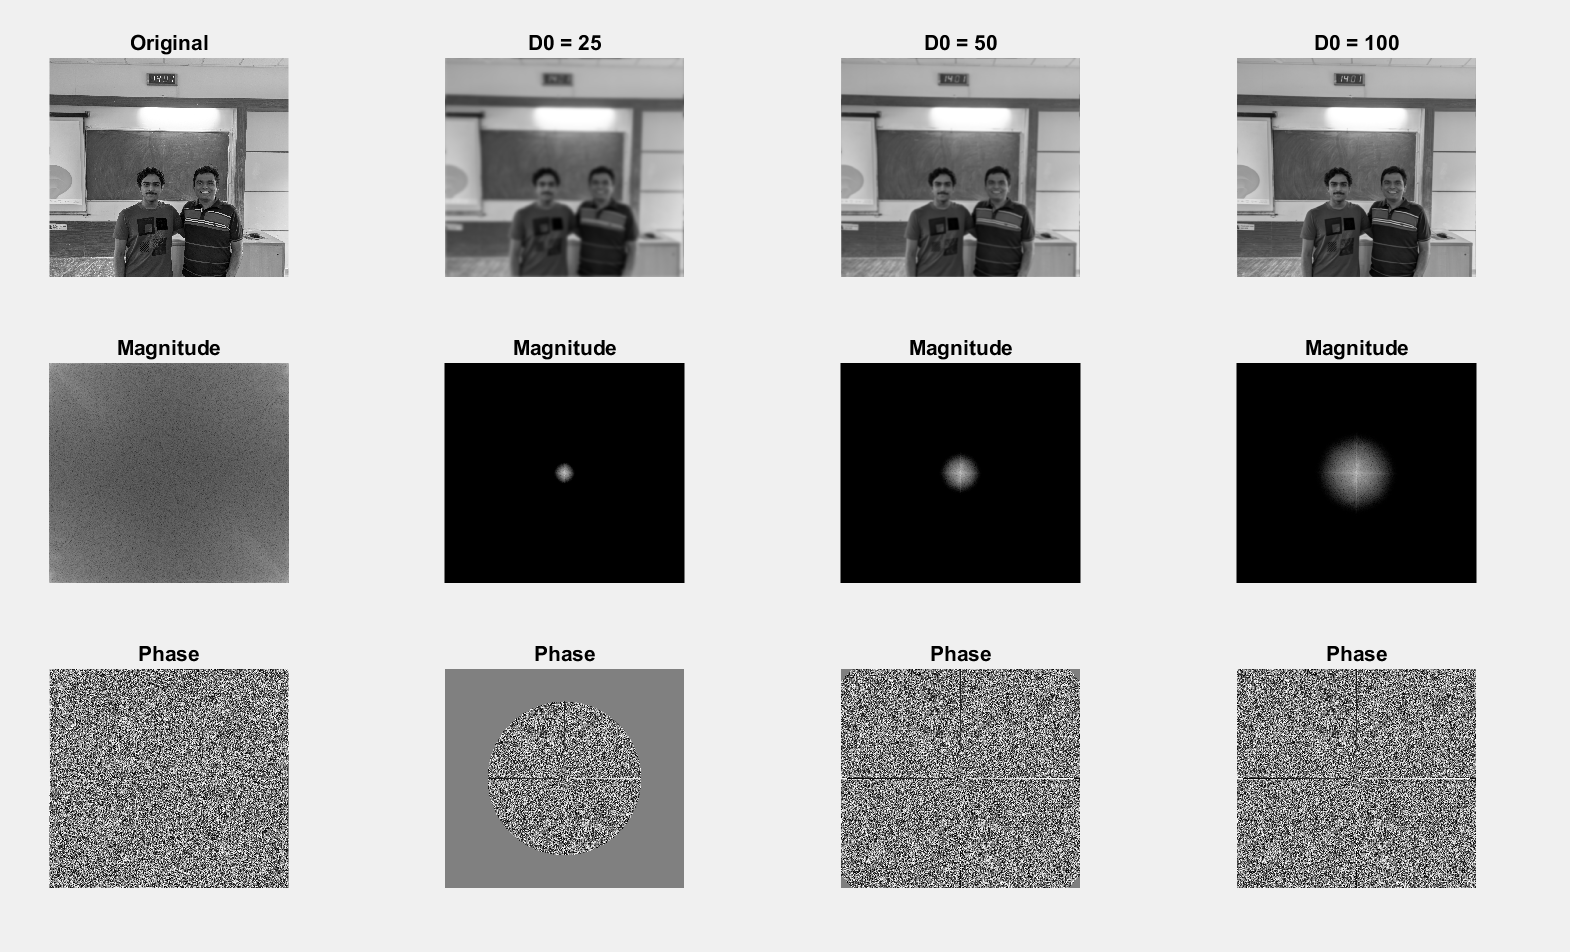
\includegraphics[width=\textwidth]{images/task2-part3.png}
	\caption{Gaussian Filtered Images of Various Sizes}
	\label{fig:gaussian lpf}
\end{figure}

The smooth nature of the Gaussian Filter can be seen in the magnitude plot of each of the images, where the central circle tapers off smoothly, rather than a sharp cutoff. As the size of the filter was increased, the image came into more focus, and more details were visible.
It's likely that a size of about 200 would be sufficient to caputre all details while ignoring high frequency noise.

\subsection{Ideal HPF}
The ideal high pass filter is defined as:
\begin{equation}
	D(u, v) = \begin{cases}
		0 \hspace*{5mm} D(u, v) < R_0 \\
		1 \hspace{5mm} D(u, v) > R_0
	\end{cases}	
\end{equation}
This filter only acts on the frequency domain, but often produces sharp ringing effects due to the high cutoff. 

\begin{figure}[h!]
	\centering
	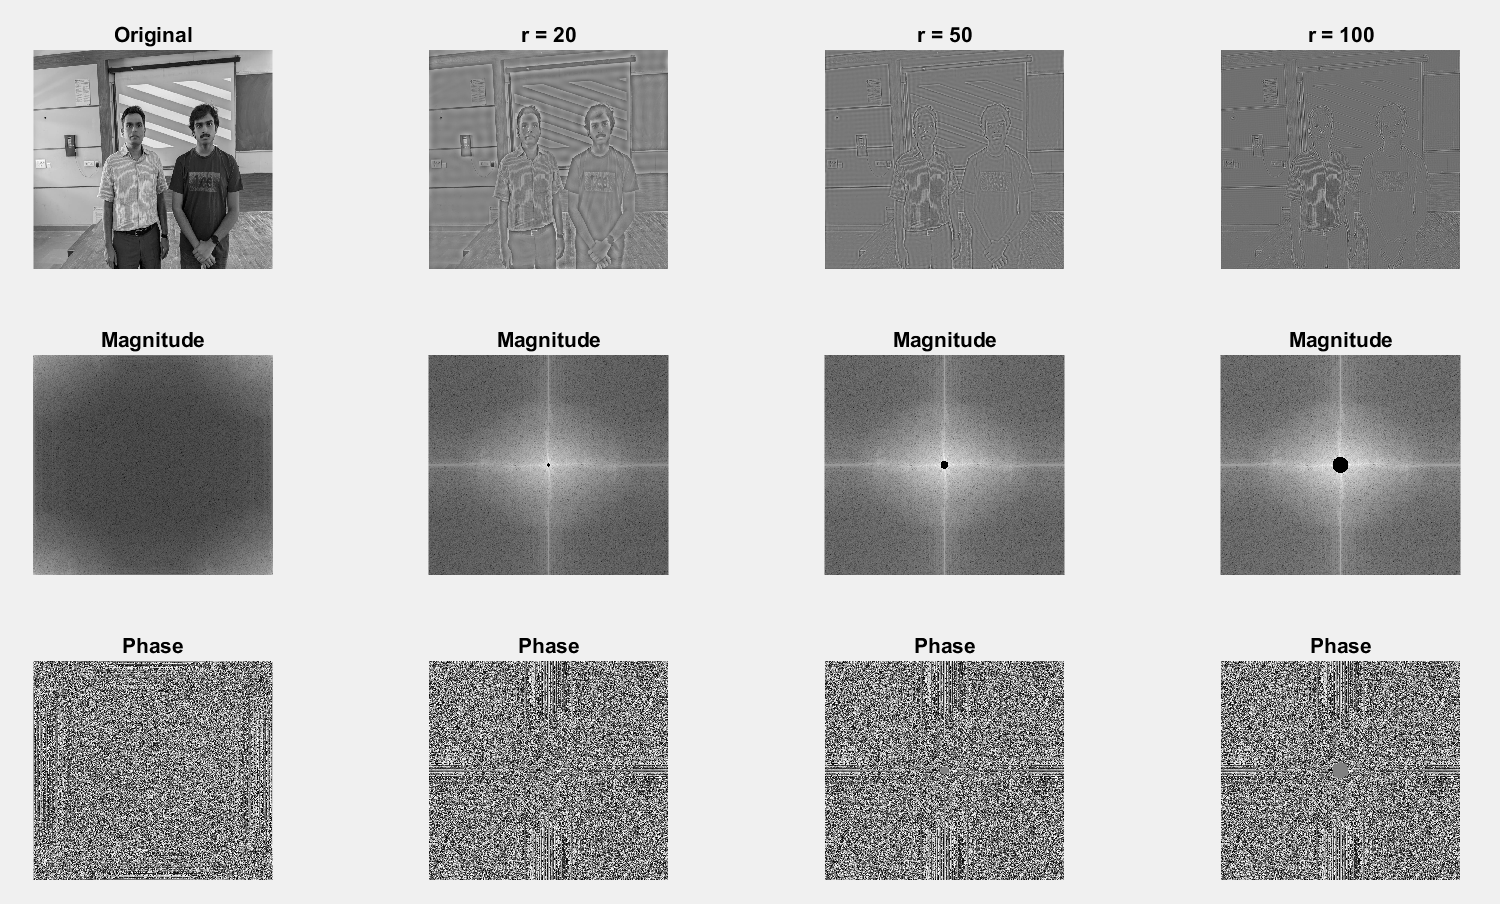
\includegraphics[width=0.85\textwidth]{images/task2-part4-circular.png}
	\caption{Ideal Circular HPF of Various Sizes}
	\label{fig:ideal circular hpf}
\end{figure}

\begin{figure}[h!]
	\centering
	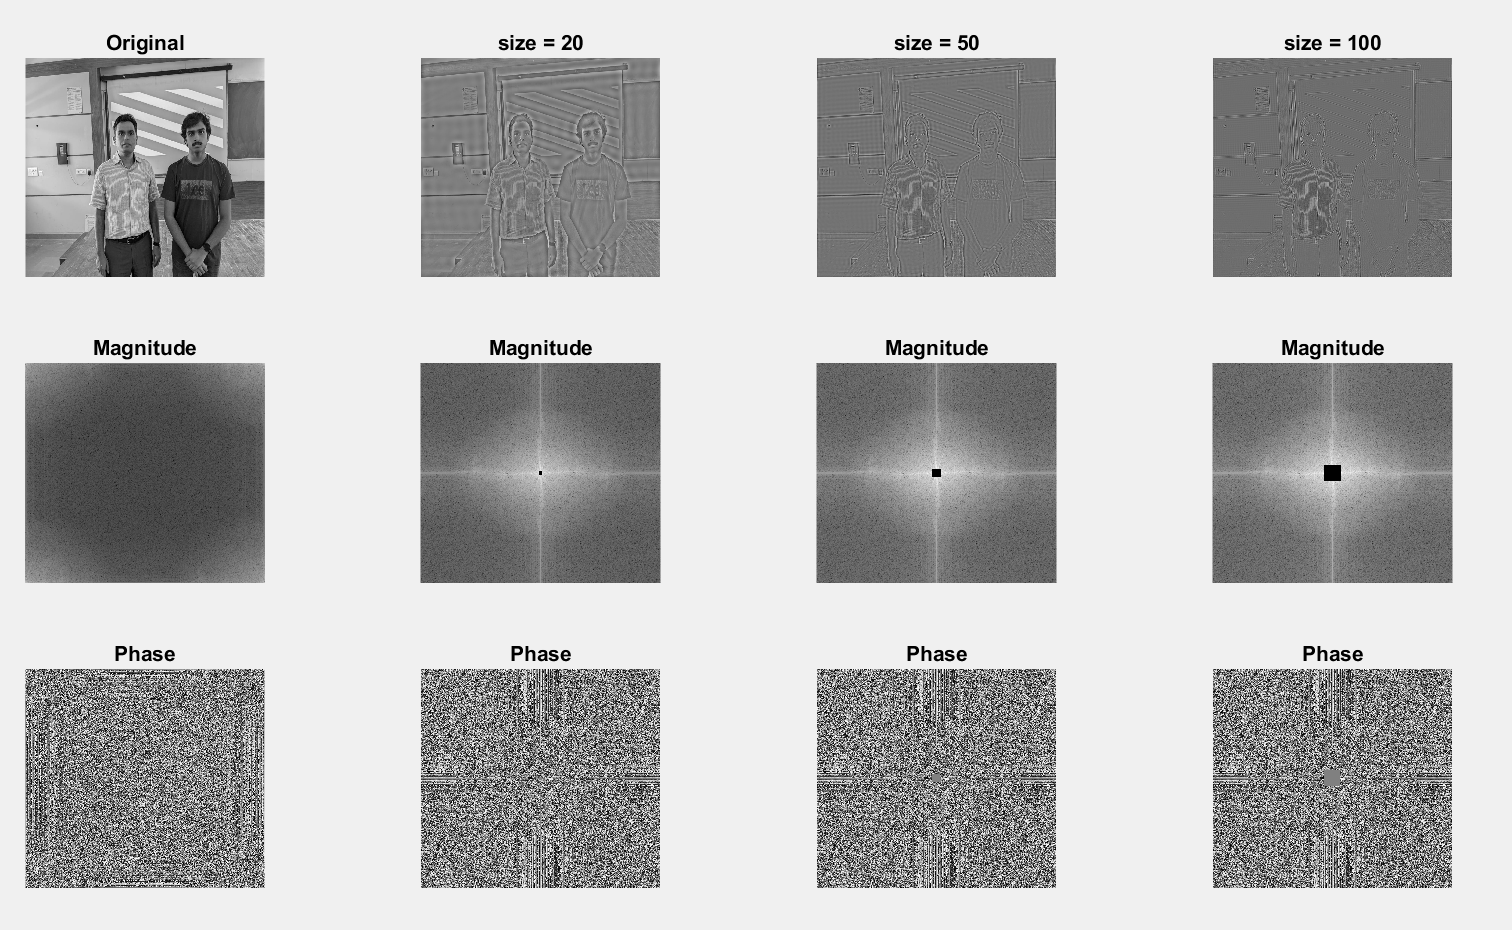
\includegraphics[width=0.85\textwidth]{images/task2-part4-rectangular.png}
	\caption{Ideal Rectangular HPF of Various Sizes}
	\label{fig:ideal rectangular hpf}
\end{figure}

Figures \ref{fig:ideal circular hpf} and \ref{fig:ideal rectangular hpf} shows the results of applying the ideal HPF with radii 20, 50 and 100 pixels. The ringing effect is very visible in the images, especially at lower radii. As the radius increases, more high frequency components are allowed through, and the image becomes clearer, but the ringing effect remains.

\subsection{Butterworth HPF}
\label{subsec:butterworth hpf}
The butterworth HPF is mathematically defined as:
\begin{equation}
	H(u, v) = \frac{1}{1 + \left(\frac{D_0}{D(u, v)}\right)^{2n}}
\end{equation}
Where $D_0$ is the cutoff frequency, and $n$ is the order of the filter. For this assignment, $n = 1, 2, 4$ was used. The same radii as before were used, and the results are shown in Figure \ref{fig:butterworth hpf}.

\begin{figure}[h!]
	\centering
	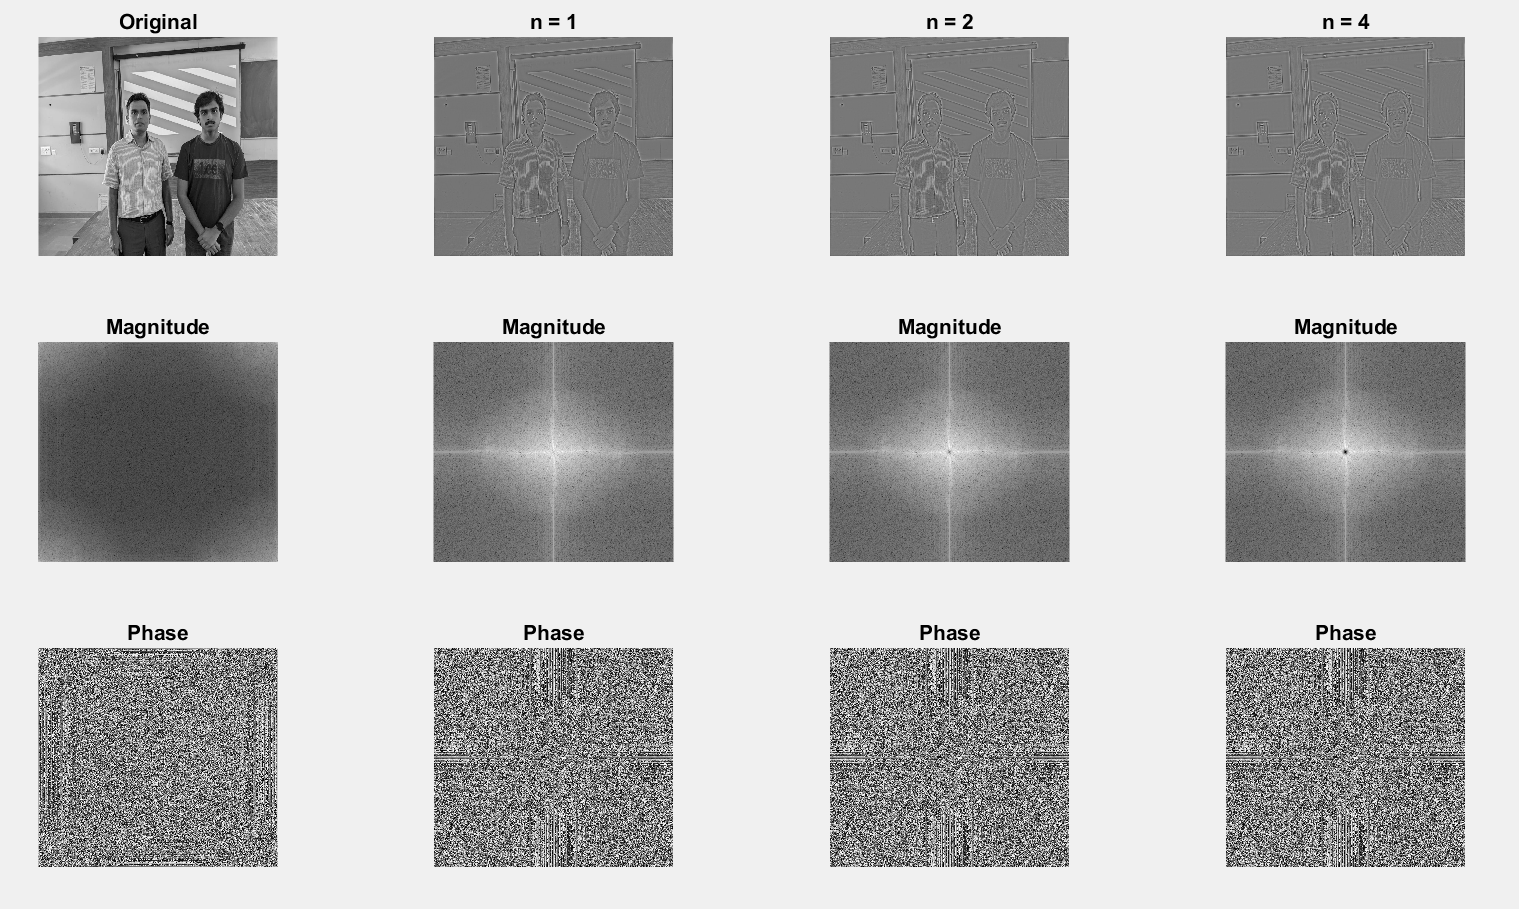
\includegraphics[width=\textwidth]{images/task2-part5.png}
	\caption{Butterworth HPF of Various Orders and Sizes}
	\label{fig:butterworth hpf}
\end{figure}

The initial image had the most noise, and as the order of the butterworth filter was increased, this noise to signal ratio went down, with signal amount going higher. This is because the main signal components are contained in the lower frequency components. The outline can be seen in these filtered images.

\newpage
\subsection{Gaussian HPF}
\label{subsec:gaussian hpf}
The Gaussian HPF is mathematically defined as:
\begin{equation}
	H(u, v) = 1 - e^{-\frac{D^2(u, v)}{2D_0^2}}
\end{equation}
Where $D_0$ is the cutoff frequency. The same radii as before were used, and the results are shown in Figure \ref{fig:gaussian hpf}. The matlab implementation is shown below.
\begin{lstlisting}[language=python]
for D0 = cutoffs
    H = 1 - exp(-(D.^2)./(2*(D0^2)));
    F_filt = fft_shifted_2 .* H;
    img_filt = real(ifft2(ifftshift(F_filt)));
    imgs1{end+1} = img_filt; F1s{end+1} = F_filt;
end
\end{lstlisting}

\begin{figure}[h!]
	\centering
	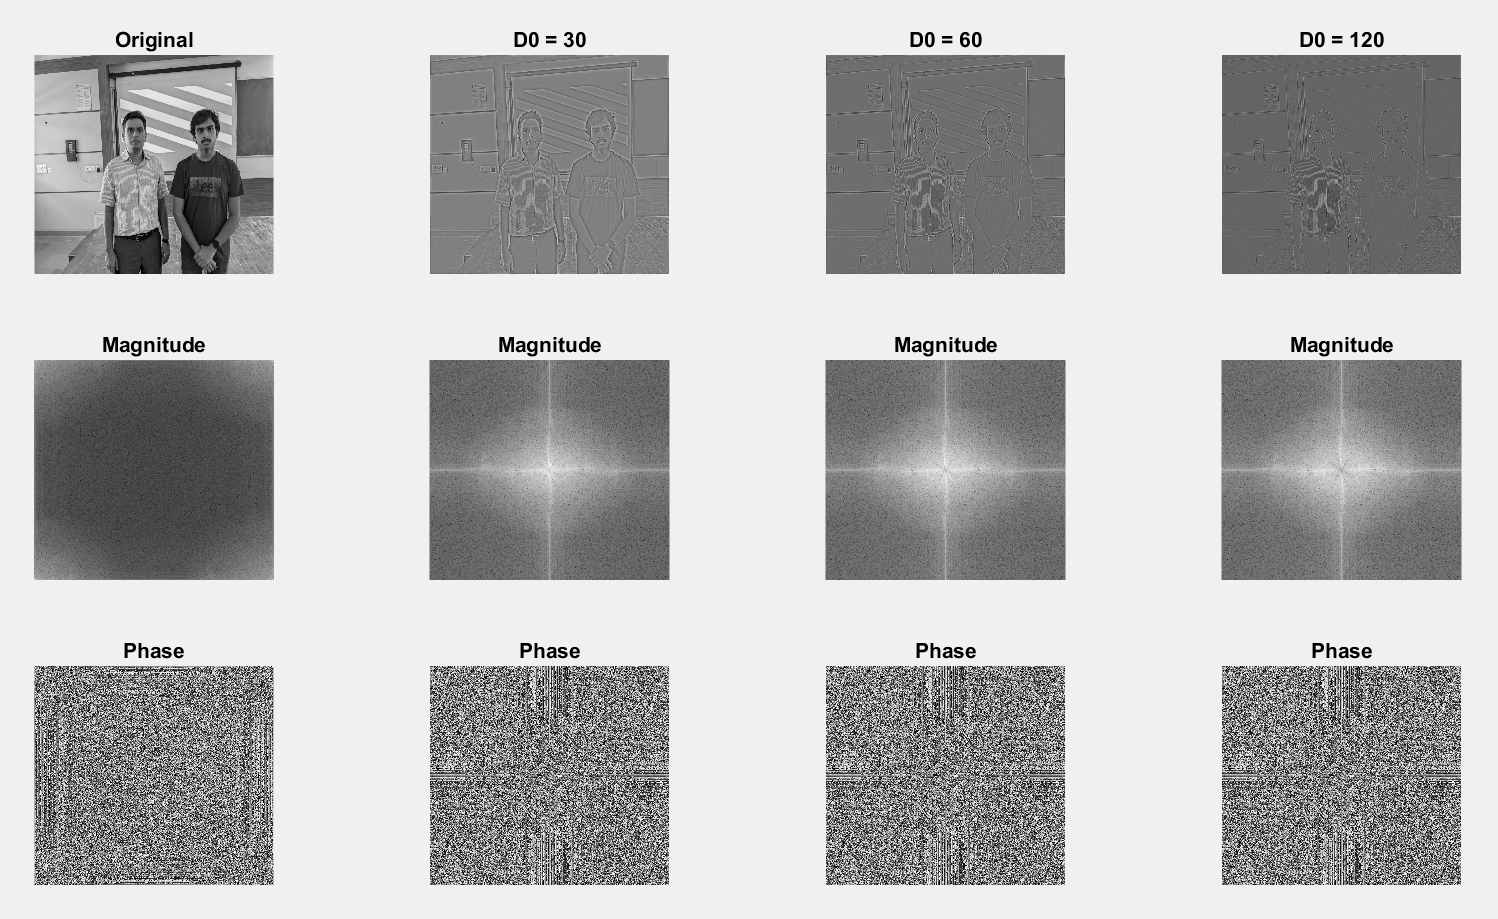
\includegraphics[width=\textwidth]{images/task2-part6.png}
	\caption{Gaussian HPF of Various Sizes}
	\label{fig:gaussian hpf}
\end{figure}

The Gaussian HPF has a smooth transition, and does not have the ringing effect that the ideal HPF has. As the size of the filter was increased, the features of the image kept reducing as expected.

\subsection{Adding and Removing Noise}
\label{sec:adding and removing noise}
The final task of this assignment was to add noise to an image, and then remove it using filtering. The following noise profile was added to the image:
\begin{lstlisting}[language=python]
    noise = noise_amp * sin(2*pi * f_noise * xgrid / N);
    I_noisy = I + noise;
\end{lstlisting}
This noise addition and removal was done on both the images.

In order to really show the difference between the filters, both an ideal LPF and a Butterworth LPF were used. A comparison can be seen on the images.

\begin{figure}[h!]
	\centering
	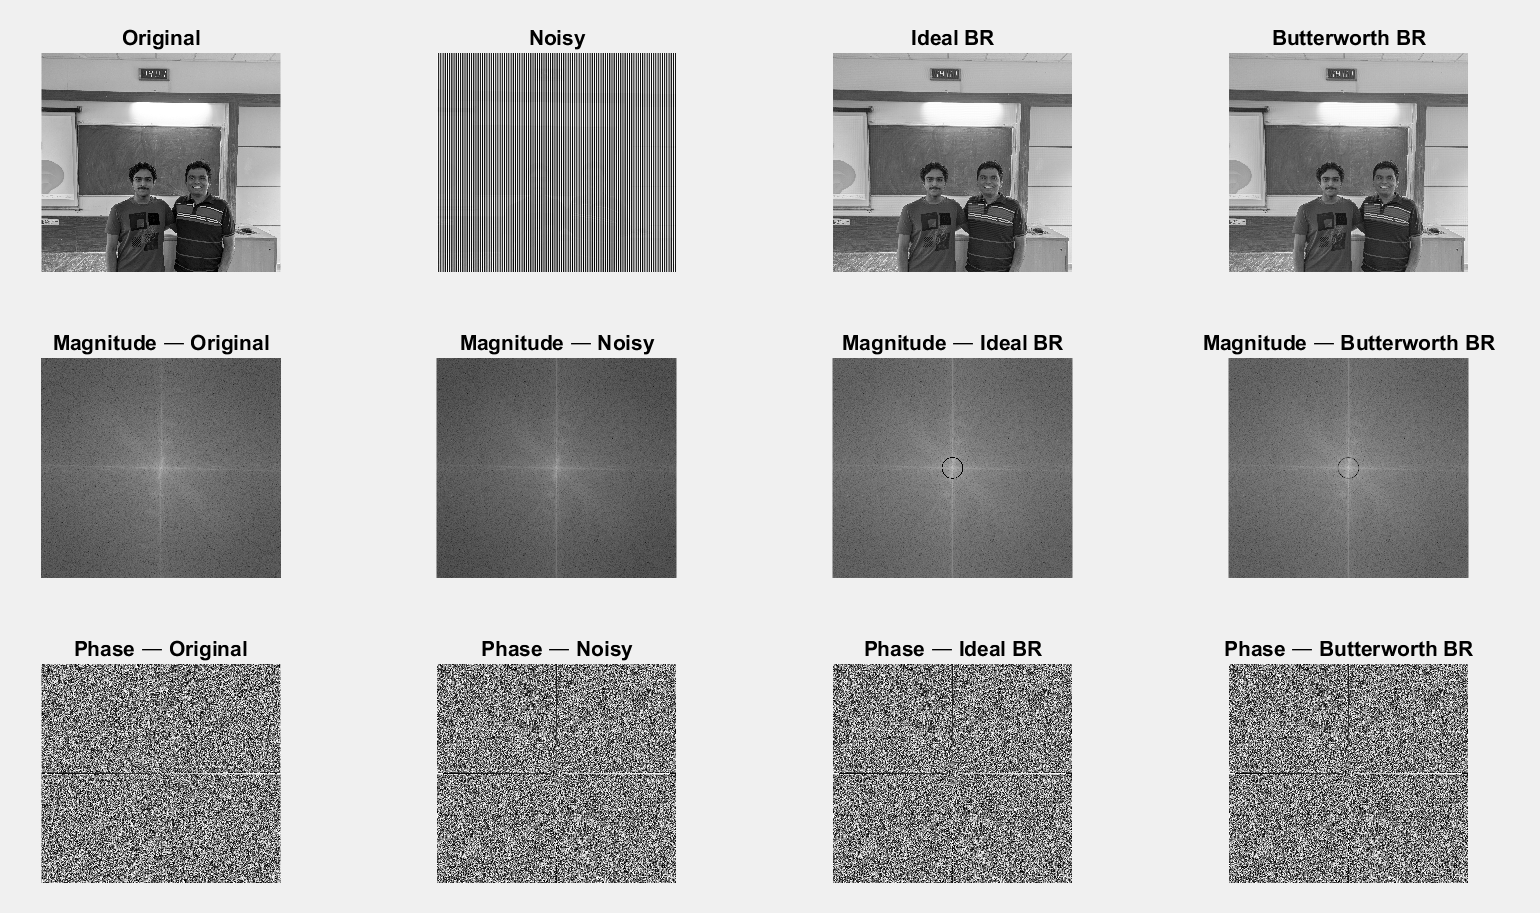
\includegraphics[width=0.81\textwidth]{images/task2-part7,8-img1.png}
	\caption{Original Image 1, Noised, Cleaned with Ideal LPF, Cleaned with Butterworth LPF}
	\label{fig:img1 noise removal}
\end{figure}

\begin{figure}[h!]
	\centering
	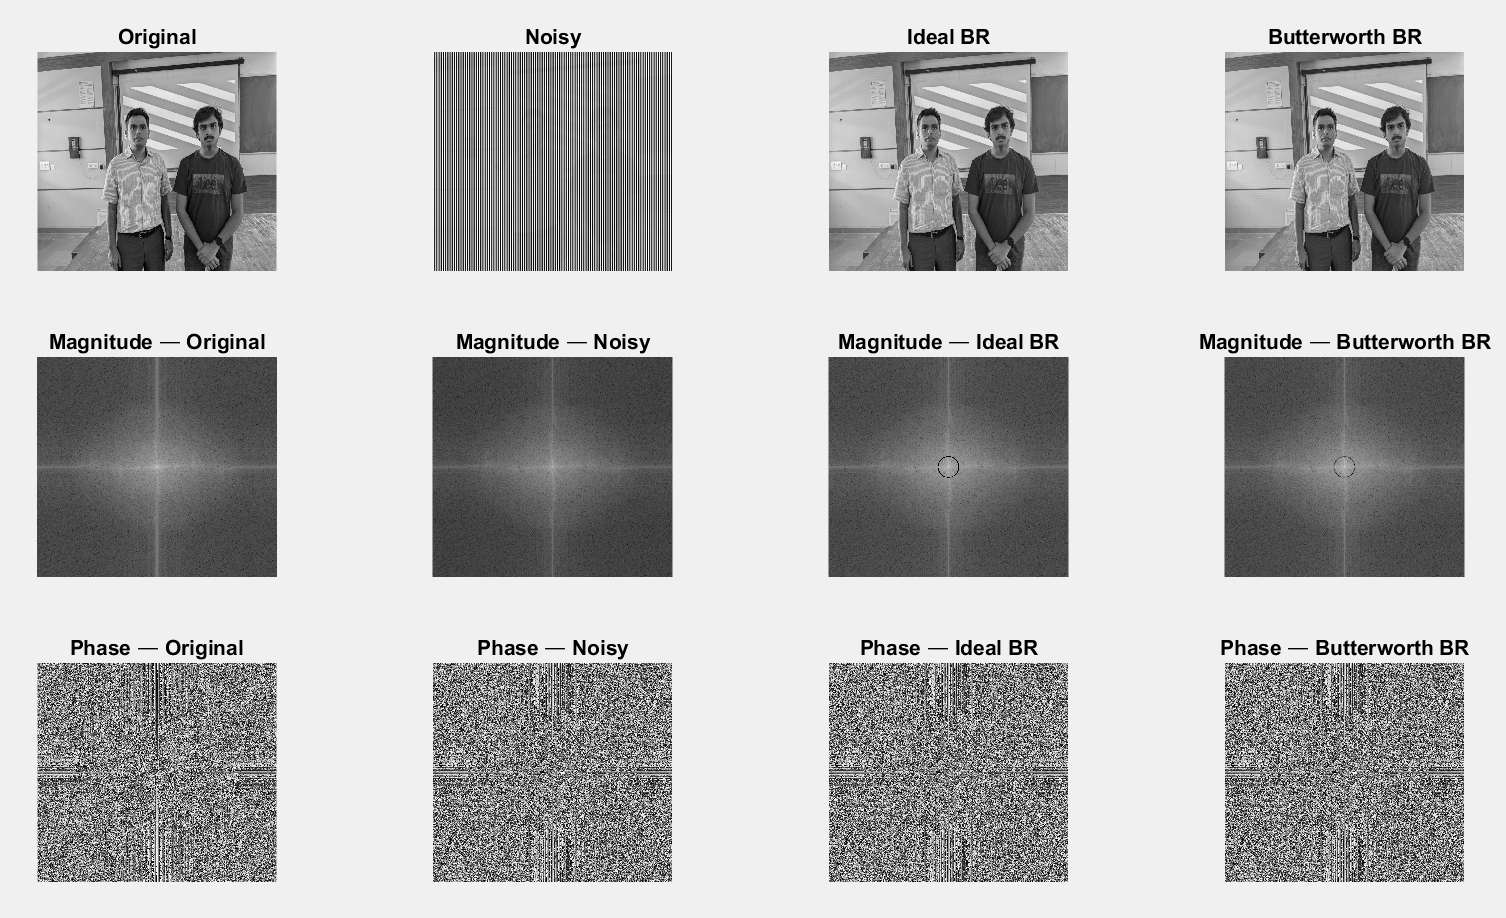
\includegraphics[width=0.81\textwidth]{images/task2-part7,8-img2.png}
	\caption{Original Image 2, Noised, Cleaned with Ideal LPF, Cleaned with Butterworth LPF}
	\label{fig:img2 noise removal}
\end{figure}

Figures \ref{fig:img1 noise removal} and \ref{fig:img2 noise removal} show the original image, the noised image, the image cleaned with an ideal LPF, and the image cleaned with a Butterworth LPF. It can be seen that both filters are able to remove the noise, but the Butterworth LPF does a better job of preserving the details of the image while removing the noise. The ideal LPF, while effective at removing noise, also removes some of the finer details of the image, leading to a loss of quality.

\newpage
\newpage
\section{Conclusion}

This assignment explored key concepts of frequency-domain image processing using MATLAB:

\begin{itemize}
    \item \textbf{Importance of Phase vs. Magnitude:} 
    \begin{itemize}
        \item Phase \(\angle F(u,v)\) contains most of the structural information in an image.
        \item Magnitude \(|F(u,v)|\) primarily determines intensity and contrast.
        \item Swapping magnitude and phase between images confirmed that phase dominates perceived structure.
    \end{itemize}
    
    \item \textbf{Spatial Transformations:} 
    \begin{itemize}
        \item Circular shifting preserves \(|F(u,v)|\) but introduces predictable phase shifts.
        \item Linear translation introduces a linear phase term in the frequency domain, changing the position of image features.
    \end{itemize}
    
    \item \textbf{Filtering:} 
    \begin{itemize}
        \item Filters selectively enhance or suppress frequency components to reduce noise or highlight details.
        \item \textbf{Ideal filters} have sharp cutoffs but can introduce ringing artifacts in the spatial domain.
        \item \textbf{Butterworth filters} smooth the transition with a tunable order \(n\), balancing detail preservation and artifact reduction.
        \item \textbf{Gaussian filters} provide the smoothest frequency response, minimizing artifacts at the cost of slight loss in sharpness.
        \item Filtering noisy images demonstrated how frequency-selective filtering can recover the underlying signal while preserving key features.
    \end{itemize}
    
    \item \textbf{Further Work:}
    \begin{itemize}
        \item Explore adaptive or anisotropic filtering techniques.
        \item Consider multi-resolution transforms, such as wavelets, for localized frequency analysis.
        \item Optimize filter parameters mathematically, e.g., by minimizing spatial-domain error metrics, for robust noise removal.
    \end{itemize}
\end{itemize}

\end{document}
